\documentclass{article}
\usepackage[utf8]{inputenc}
\usepackage{geometry}
\usepackage{datetime2}
\usepackage{xparse}
\usepackage{amsmath}
\usepackage{booktabs}
\usepackage{array}
\usepackage{hyperref}


 \geometry{
 a4paper,
 total={170mm,257mm},
 left=20mm,
 top=20mm,
 }

 
 \usepackage{graphicx}
 \usepackage{titling}

 \title{Fuzzification of Room Temperature 
}
\date{18 March 2025}
 
 \usepackage{fancyhdr}
\fancypagestyle{plain}{%  the preset of fancyhdr 
    \fancyhf{} % clear all header and footer fields
    \fancyfoot[R]{}
    \fancyfoot[L]{}
    \fancyhead[L]{
\includegraphics[width=2cm]{ITS_pojok.pdf}}
    \fancyhead[R]{ \DTMnow}
}
\makeatletter
\def\@maketitle{%
  \newpage
  \null
  \vskip 1em%
  \begin{center}%
  \let \footnote \thanks
    {\LARGE \@title \par}%
    \vskip 1em%
    %{\large \@date}%
  \end{center}%
  \par
  \vskip 1em}
\makeatother

\usepackage{lipsum}  
% \usepackage{cmbright} % Change the font by zee

\begin{document}

\maketitle


\noindent\begin{tabular}{l @{ : } l}
        Nama                &  Septian Feter Arifianto \\  
        NIM                 &  6022251072 \\  
        Teacher             &  Muhammad Qomaruz Zaman, S.T., M.T., Ph.D.\\
        Mata Kuliah         &  Kecerdasan Buatan Assigment 2 \\
\vspace{0,2cm}
        Class name          &  Kelas X\\
        GitHub Link & \url{https://github.com/septianfeter-arifianto/assigment-2.git}\\
\end{tabular}
\vspace{1cm}

\section*{1. Inisialisasi Lingkungan dan Pembuatan Fungsi Membership}
Langkah awal dalam proyek ini adalah menyiapkan pustaka pendukung yaitu NumPy untuk manipulasi array numerik dan Matplotlib untuk memvisualisasikan data. Inti dari proses fuzifikasi ini terletak pada pembuatan fungsi kustom bernama triangle. Fungsi ini dirancang untuk mengubah nilai tegas (crisp) menjadi nilai linguistik dengan logika if/elif/else. Di dalam fungsi ini, diterapkan perhitungan matematis untuk menentukan posisi nilai $x$ terhadap batas-batas segitiga ($a, b, c$) guna menghasilkan derajat keanggotaan antara 0 hingga 1.

\section*{2. Penentuan Parameter dan Ruang Lingkup Data}
Setelah fungsi dasar terbentuk, tahap selanjutnya adalah menetapkan variabel kontrol yaitu suhu air sebesar $32.5^\circ C$ sebagai data yang akan diuji. Untuk menciptakan grafik yang halus, dibuatlah sebuah ruang sampel data menggunakan np.linspace(10, 40, 1000). Angka ini merepresentasikan rentang temperatur t dari $10^\circ C$ hingga $40^\circ C$ yang akan dipetakan ke dalam koordinat sumbu X pada grafik fuzifikasi


\section*{3. Pemodelan Variabel Linguistik (Fuzifikasi)}
Proses ini membagi rentang suhu menjadi tiga kategori utama dengan karakteristik kurva yang berbeda:
\begin{itemize}
    \item Himpunan Dingin: Didefinisikan dengan titik (15, 15, 25), di mana suhu di bawah 15 memiliki keanggotaan penuh (1.0) dan mulai menurun secara linear hingga mencapai 0 pada suhu $25^\circ C$
    \item Menggunakan model segitiga simetris (15, 25, 35). Pada tahap ini, suhu $25^\circ C$ merupakan titik puncak (1.0), sedangkan suhu $32.5^\circ C$ akan dihitung posisinya pada garis menurun menuju $35^\circ C$.
    \item Dirancang dengan parameter (25, 35, 35) di mana nilai keanggotaan mulai tumbuh dari 0 pada suhu $25^\circ C$ dan tetap berada di angka 1.0 (maksimal) setelah melewati suhu $35^\circ C$.
\end{itemize}

\section*{4. Visualisasi Data dan Anotasi Teknis}
Tahap akhir adalah merangkai semua data tersebut ke dalam representasi visual yang informatif. Kode menggunakan perintah plt.plot untuk menggambar kurva keanggotaan dengan warna pembeda: merah untuk dingin, hijau untuk sedang, dan biru untuk panas.
\begin{itemize}
    \item Garis Penanda (Axvline): Garis putus-putus oranye ditarik secara vertikal tepat pada posisi $32.5$ untuk menunjukkan di mana posisi input berada terhadap ketiga kurva tersebut.
    \item Anotasi Dinamis: Menggunakan fungsi plt.text untuk menampilkan nilai numerik "t = 32.5" secara langsung di dalam grafik, memberikan kejelasan instan bagi pembaca
    \item Simbol Matematika: Label sumbu Y diformat menggunakan sintaks LaTeX r'$\mu_s(t)$' untuk menampilkan simbol standar fuzifikasi secara profesional.
\end{itemize}
Narasi ini menggambarkan bagaimana sebuah nilai suhu mentah diproses melalui logika matematika hingga menjadi informasi derajat keanggotaan yang siap digunakan.

\section*{5. Visualisasi}
\subsection*{a. Fuzzification of Room Temperature Dingin}
\begin{figure}[htbp]
    \centering
    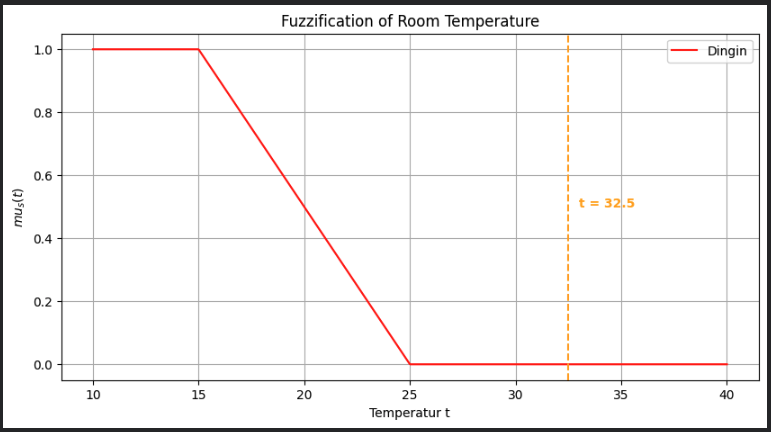
\includegraphics[width=0.5\linewidth]{Dingin.png}
    \caption{Dingin}
    \label{fig:enter-label}
\end{figure}
\subsection*{b. Fuzzification of Room Temperature Sedang}
\begin{figure}[htbp]
    \centering
    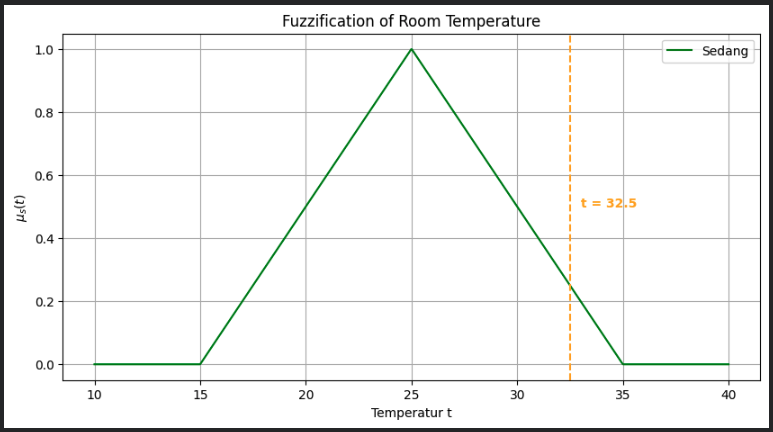
\includegraphics[width=0.5\linewidth]{Sedang.png}
    \caption{Sedang}
    \label{fig:enter-label}
\end{figure}
\subsection*{c. Fuzzification of Room Temperature Panas}
\begin{figure}[htbp]
    \centering
    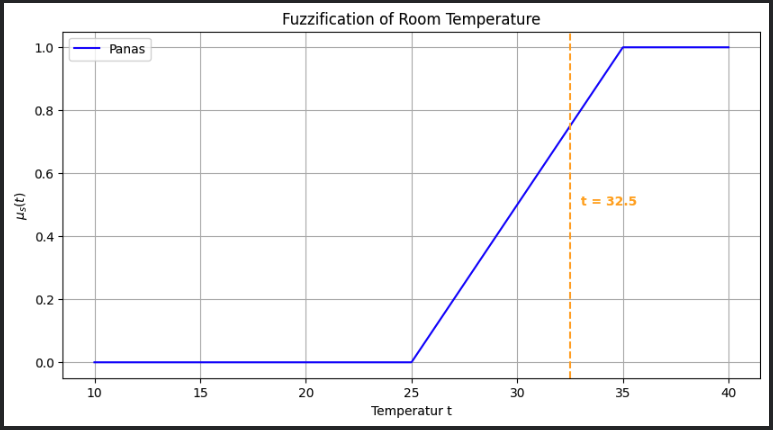
\includegraphics[width=0.5\linewidth]{Panas.png}
    \caption{Panas}
    \label{fig:enter-label}
\end{figure}
\end{document}
